On peut observer nos prédictions sur le jeu de test en entraînant notre modèle sur le jeu d'entraînement au complet. Voici les 30 premières prédictions:

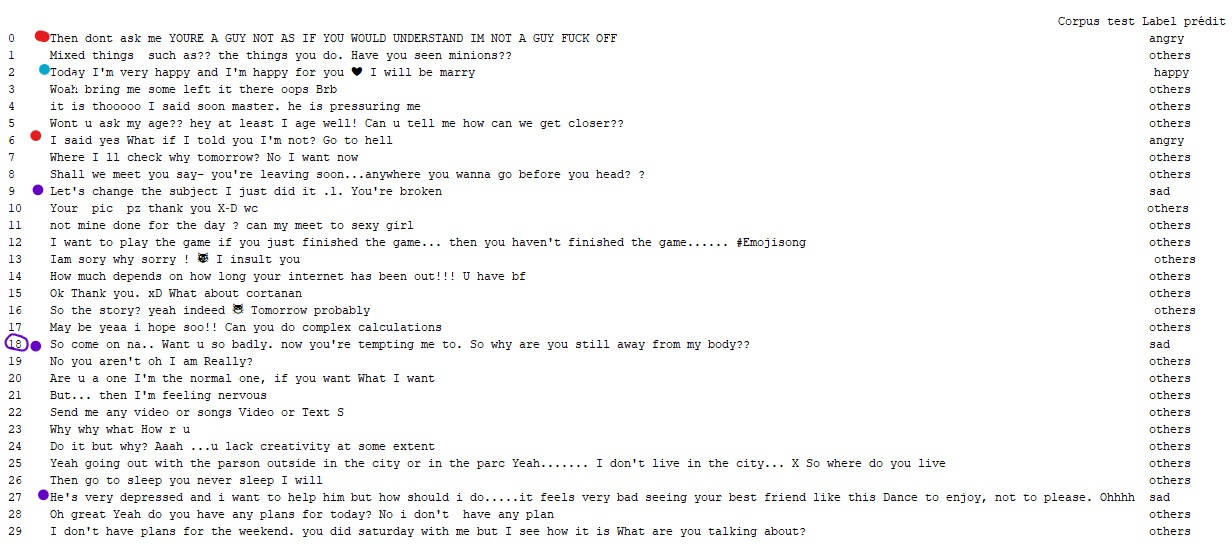
\includegraphics[width=\linewidth,keepaspectratio]{images/couleur_predictions}

Il est difficile d'analyser facilement nos prédictions puisqu'on n'a pas les classes à notre disposition. 

On peut toutefois voir qu'à tous ceux pour lesquels on prédit soit happy/angry/sad, les prédictions semblent bonnes sauf pour le numéro 18 qui n'a clairement pas l'air triste. On peut supposer que cet échange cocasse est mal classé à cause de "Want u so badly". En effet, le mot \emph{"badly"} a une forte connotation négative, ce qui induit notre modèle à classer ce texte en tant que triste. 

En regardant rapidement, on peut voir que ceux classés comme \emph{others} ont l'air particulièrement neutre, sauf peut-être le 13, mais cela est assez subjectif.

Ce petit échantillon nous laisse avec une très bonne impression de notre modèle.